\section{Implementation Workflow}

The workflow for generating CoreDSL code from OSAL files, as depicted in Figure 4.1, involves several key stages that transform input operations into CoreDSL code suitable for integration into M2-ISA-R. The overall flow can be divided into the following steps:

\begin{enumerate}
    \item \textbf{Parsing the OSAL Files:} The process begins with the input OSAL (Operation Set Architecture Language) files, which contain the operation definitions. These files are processed by an XML Parser that extracts the operation properties and relevant data.

    \item \textbf{Filtering Operations:} Once parsed, the operations undergo a filtering stage. Here, multiple criteria are applied, such as the number of inputs and outputs, whether the operation has side effects, and other predefined properties. These conditions help identify which operations are suitable for further processing.

    \item \textbf{Handling Single Execution Operations:} If the operation is determined to be a single execution type (i.e., simple operations that can be executed in a single step), it is immediately passed to the transformation stage. For non-single execution operations, a base operation is identified and combined with other operations as needed before continuing the process.

    \item \textbf{Transforming to CoreDSL:} The filtered and combined operations are transformed into CoreDSL. This step includes encoding the behavioral aspects of the operation into a format compatible with the CoreDSL language, facilitating its integration into the larger ISA model.

    \item \textbf{Auto Encoding and Assembly:} Alongside the behavioral encoding, the process includes an automated stage for encoding and assembly generation. This ensures that the operations are fully represented in both the abstract behavioral sense and in terms of the machine-level encoding required for execution.

    \item \textbf{Code Generation:} A CoreDSL template is used to guide the generation of the final code. The CoreDSL template serves as a scaffold, ensuring consistency and completeness in the generated output.

    \item \textbf{Final Code Writing:} The processed operations, including the behavior and encoding information, are passed to the writer. The writer generates the final CoreDSL code, which represents the operations in a format that is ready for integration into M2-ISA-R.

\end{enumerate}

This workflow ensures a structured and efficient transformation of OSAL files into CoreDSL code, leveraging automated encoding and assembly processes to streamline the generation of instruction set architectures for custom CPU designs.

\begin{figure}[h]
  \centering
  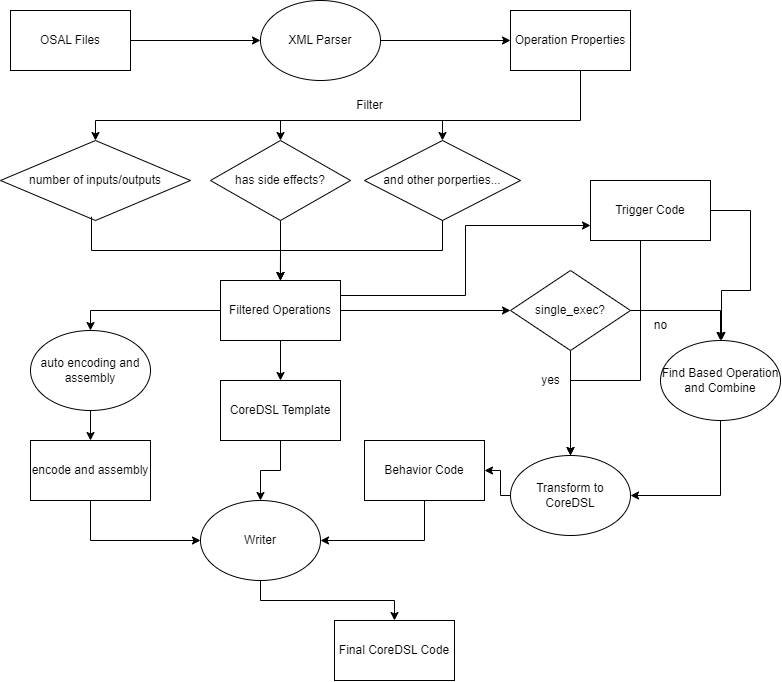
\includegraphics[width=\linewidth]{figures/flow.png}
  \caption{Implementation Flow}
\end{figure}

\section{XML Parser}

As mentioned in the previous section, OpenASIP uses XML to define the properties and semantics of custom operations.
To translate these operations into CoreDSL, we need to parse the XML representation and extract the necessary information.
We developed an XML parser based on pandas package in Python to read the XML files and extract the operation details.


\section{Operation Filtering}

\section{CoreDSL Template Generation}

\section{Behavior Code Generation}